\documentclass{article}
\usepackage{graphicx}
\usepackage{multirow}

\usepackage{siunitx}
\sisetup{
	round-mode= places,
	round-precision=2,
}

\begin{document}
	\begin{table}[h!]
		\begin{center}
			\caption{Multirow table.}
			\label{tab:table1}
			\begin{tabular}{l|S|r}
				\hline
				\textbf{Value 1} & \textbf{Value 2} & \textbf{Value 3}\\
				$\alpha$ & $\beta$ & $\gamma$ \\
				\hline
				\multirow{2}{*}{12} & 1110.1 & a\\
				& 10.1 & b\\
				\hline
				14 & 25.113231 & 
				\multirow{2}{*}{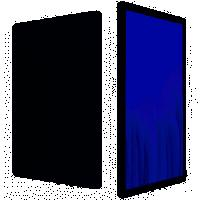
\includegraphics[width=0.07\linewidth]{picture2.jpg}}\\
				25 & 345.113231  &  \\
				\hline
				36 & 35.123531  & c \\
				\hline
			\end{tabular}
		\end{center}
	\end{table}
\end{document}